%------------------------------------------------------------------------
\hypertarget{cv:eliminarPrecondicion}{\section{Eliminar Precondición}} \label{sec:eliminarPrecondicion}

	Esta funcionalidad le permitirá eliminar una precondición innecesaria o incorrecta. 

		\subsection{Procedimiento}

			%Pasos de procedimiento
			\begin{enumerate}
	
			\item Oprima el botón \IUBotonEliminar{} de un registro existente de la pantalla \ref{fig:GestionarPrecondiciones} ''Gestionar Precondiciones''.
	
			\item Se mostrará el mensaje \ref{fig:confirmaEliminaPre} sobre la pantalla \ref{fig:GestionarPrecondiciones} ''Gestionar Precondiciones''.
			
			%Pantalla
			\begin{figure}[htbp!]
				\begin{center}
					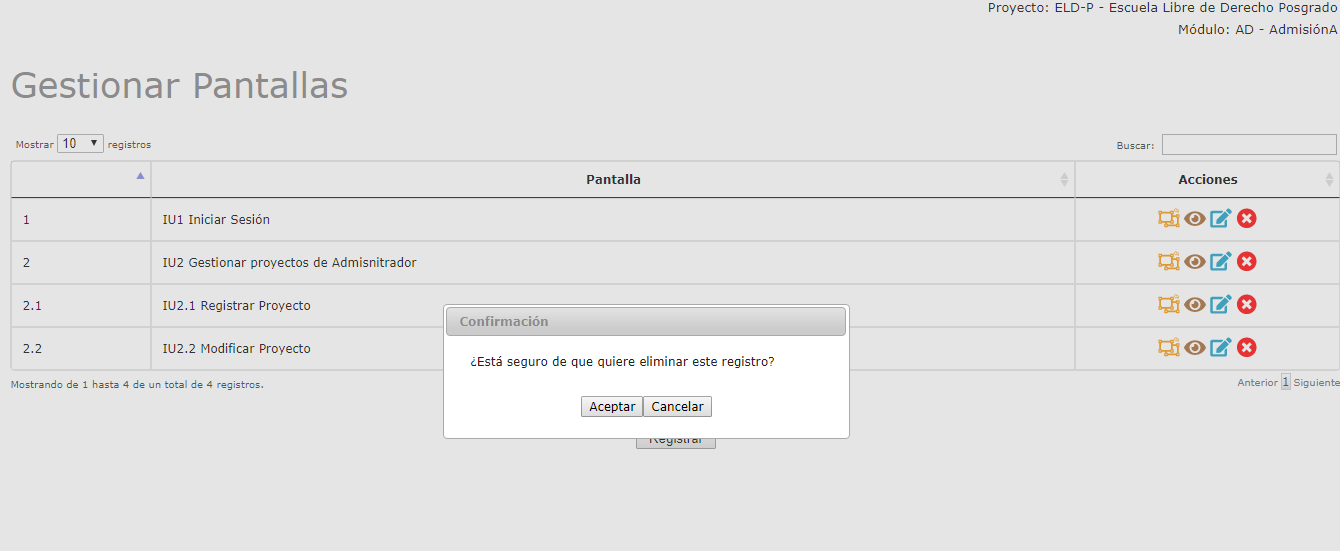
\includegraphics[scale=0.5]{roles/lider/casosUso/pantallas/IU11-3MSG10}
					\caption{MSG de Confirmación}
					\label{fig:confirmaEliminaPre}
				\end{center}
			\end{figure}
						
			\item Oprima el botón \IUAceptar.
			
			\item Se mostrará el mensaje \ref{fig:PreEliminada} en la pantalla \ref{fig:GestionarPrecondiciones} ''Gestionar Precondiciones''.
			
			\begin{figure}[htbp!]
				\begin{center}
					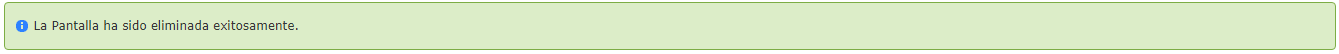
\includegraphics[scale=0.5]{roles/lider/pantallas/pantallas/IU11-3MSG1}
					\caption{MSG: Precondición Eliminada}
					\label{fig:PreEliminada}
				\end{center}
			\end{figure}
			\end{enumerate}